% Titelbereich nach dem Versuchsskript "Bildgebende Verfahren -
% Magnetresonanztomographie". Logo und MRT-Foto sind unveränderte
% Bildressourcen aus der ersten PDF-Seite; die Kennzeichnung ist angepasst.
% Das Deckblatt ist unnummeriert. Die Scan-Anleitung beginnt danach bei 1.
\hypersetup{pageanchor=false}
\begin{titlepage}
\thispagestyle{empty}
\pdfbookmark[0]{Versuchsdurchführung}{deckblatt}
\definecolor{deckblattblau}{HTML}{00549F}
\definecolor{deckblattgrau}{HTML}{666666}
\begin{tikzpicture}[remember picture,overlay]
  \node[anchor=north west,inner sep=0pt]
    at ([xshift=64.03mm,yshift=-31.06mm]current page.north west)
    {
\includegraphics[width=125.94mm]{deckblatt_logo.png}};

  \node[anchor=north west,inner sep=0pt,text=deckblattgrau,
        font={\fontfamily{phv}\fontsize{12bp}{14bp}\selectfont}]
    at ([xshift=25.4mm,yshift=-75.20mm]current page.north west)
    {Praktikum Medizintechnik - Versuchsdurchführung};

  \node[anchor=north west,inner sep=0pt,text=deckblattblau,
        font={\fontfamily{phv}\fontsize{26bp}{31bp}\selectfont\bfseries}]
    at ([xshift=25.4mm,yshift=-83.40mm]current page.north west)
    {Magnetresonanztomographie};

  \node[anchor=north west,inner sep=0pt,align=left,text=deckblattblau,
        font={\fontfamily{phv}\fontsize{23bp}{30.415bp}\selectfont}]
    at ([xshift=25.4mm,yshift=-95.40mm]current page.north west)
    {Fett-Wasser-Trennung mit der Dixon-\\Methode am 1.5 Tesla MRT};

  \node[anchor=north west,inner sep=0pt]
    at ([xshift=25.93mm,yshift=-121.28mm]current page.north west)
    {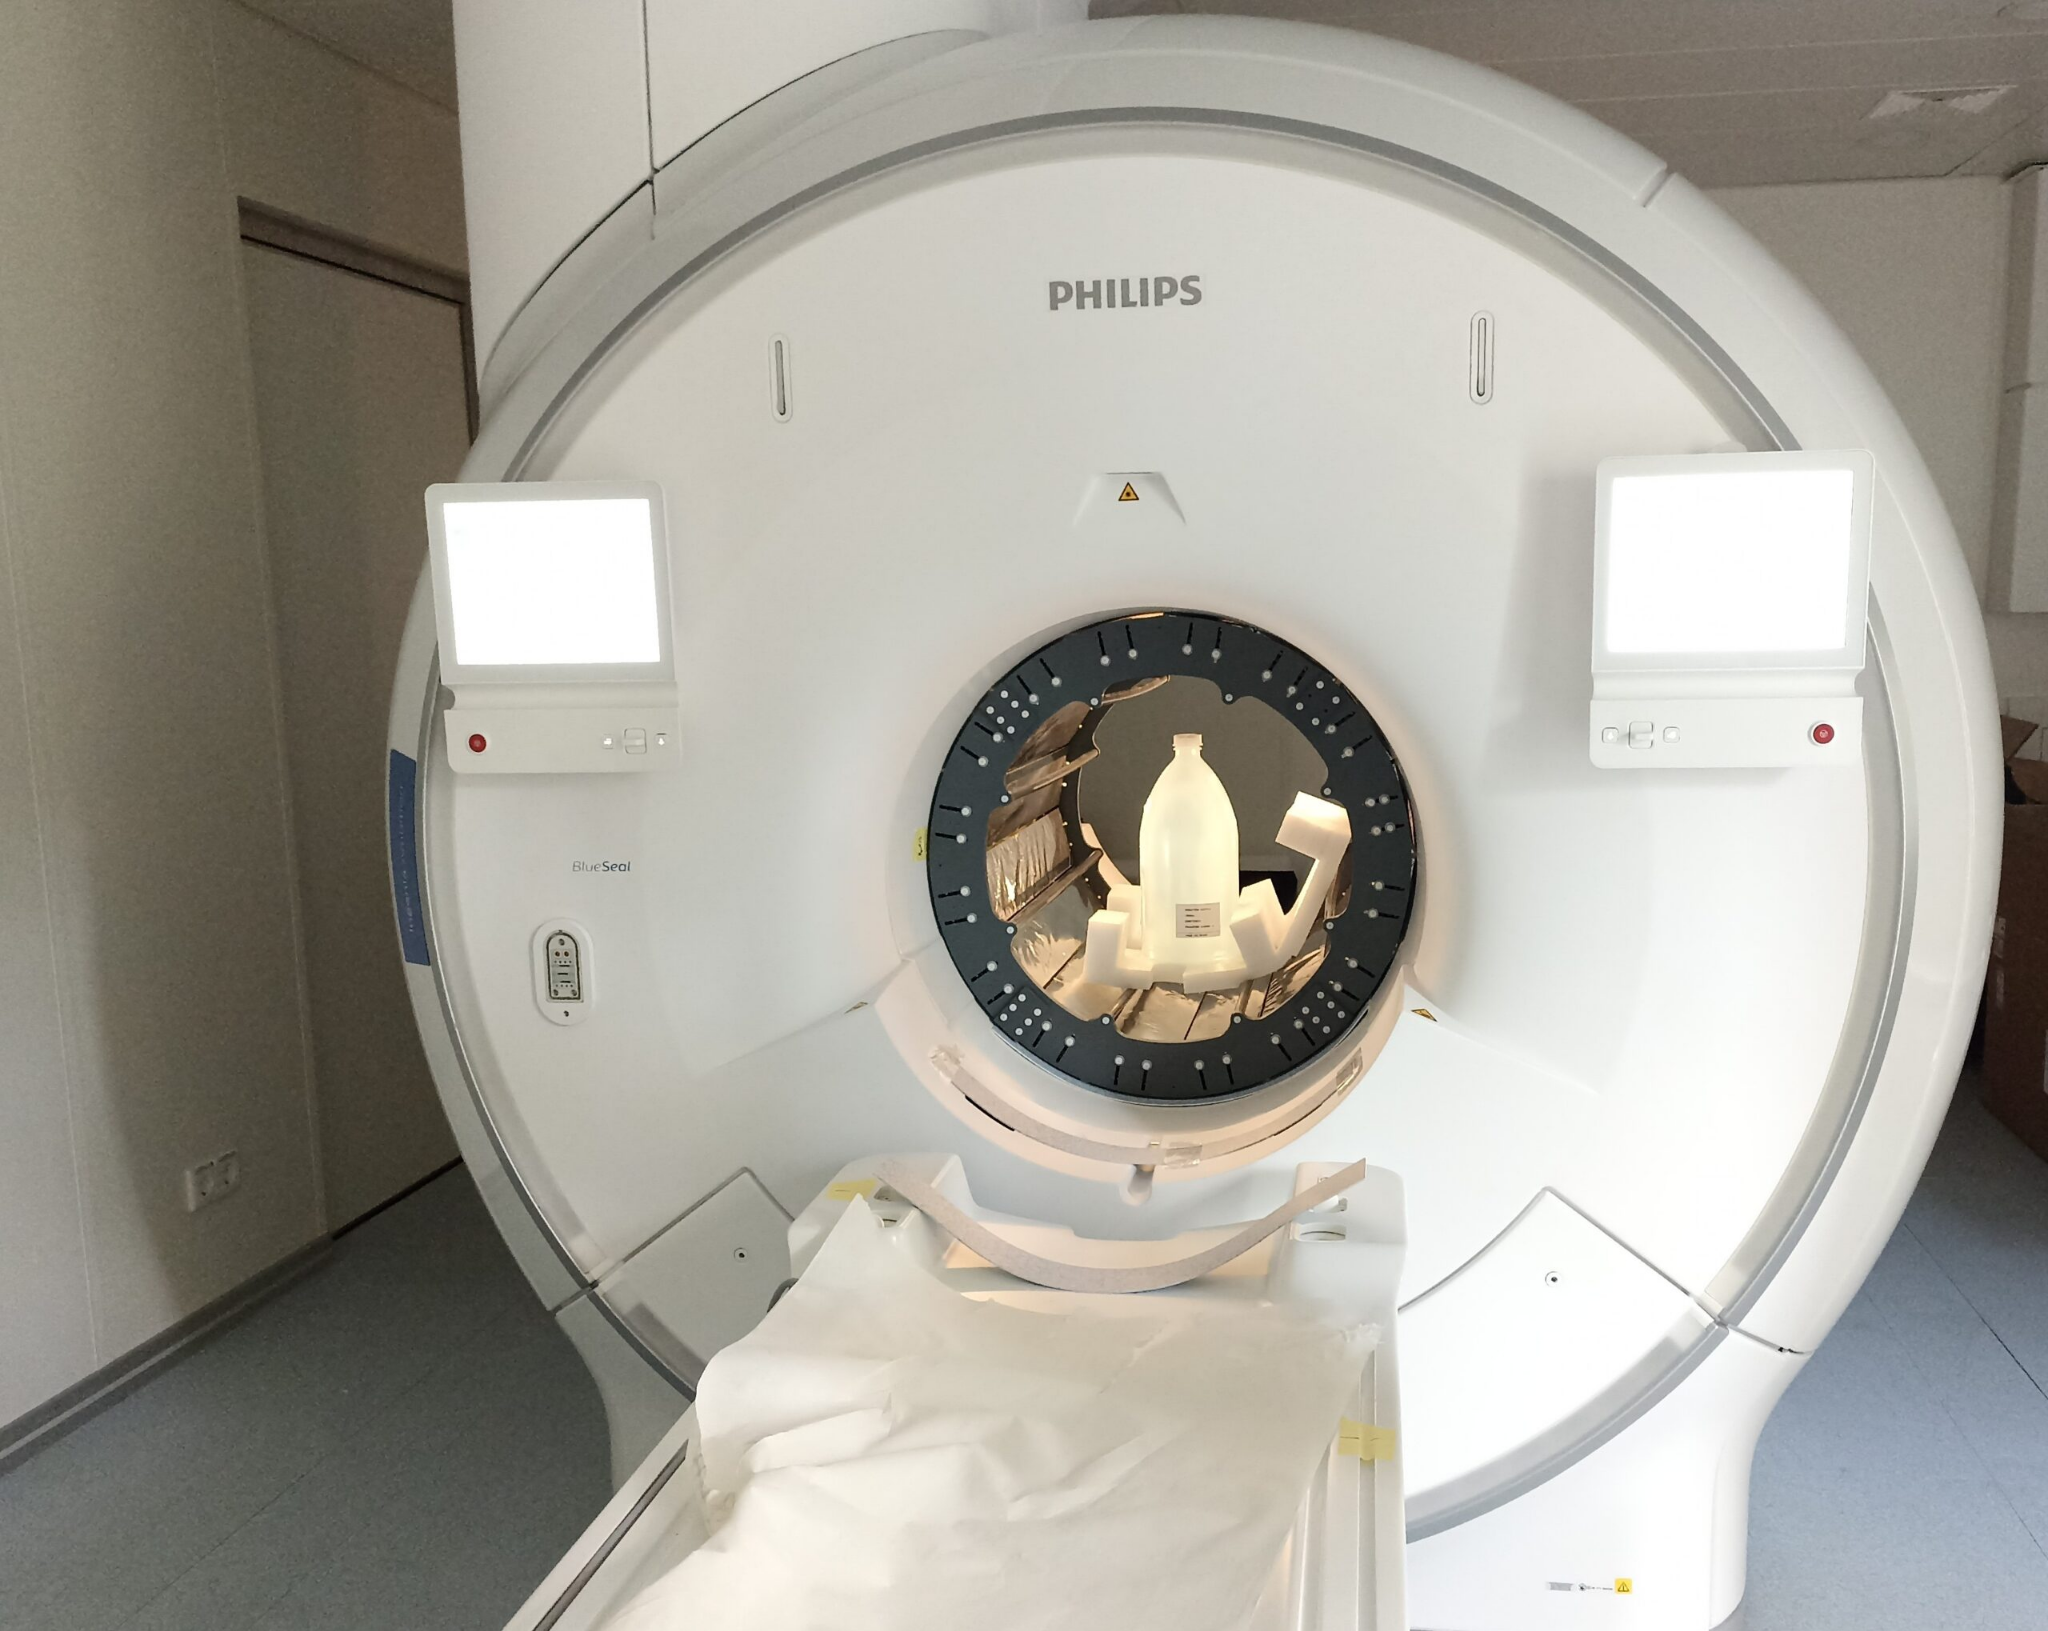
\includegraphics[width=88.64mm]{deckblatt_mrt.png}};
\end{tikzpicture}
\null
\end{titlepage}
\hypersetup{pageanchor=true}
